% Created 2020-01-28 Tue 14:57
% Intended LaTeX compiler: pdflatex
\documentclass[11pt]{article}
\usepackage[utf8]{inputenc}
\usepackage[T1]{fontenc}
\usepackage{graphicx}
\usepackage{grffile}
\usepackage{longtable}
\usepackage{wrapfig}
\usepackage{rotating}
\usepackage[normalem]{ulem}
\usepackage{amsmath}
\usepackage{textcomp}
\usepackage{amssymb}
\usepackage{capt-of}
\usepackage{hyperref}
\author{Denver Ellis}
\date{\today}
\title{}
\hypersetup{
 pdfauthor={Denver Ellis},
 pdftitle={},
 pdfkeywords={},
 pdfsubject={},
 pdfcreator={Emacs 26.3 (Org mode 9.1.9)}, 
 pdflang={English}}
\begin{document}

\tableofcontents

\section{Problem 1:}
\label{sec:org8e0957a}
Consider the following data on types of health complaint (J joint swelling, F fatigue, B back pain, M muscle weakness, C coughing, N nose running/ irritation, O other) made by tree planters. Obtain frequencies and relative frequencies for the various categories, and draw a bar chart. (The data is consistent with percentages given in the article “Physiological Effects of Work Stress and Pesticide Exposure in Tree Planting by British Columbia Silviculture Workers,” Ergonomics, 1993: 951–961.)

\subsection{Frequency:}
\label{sec:org71ff32d}
\begin{itemize}
\item B= 7
\item C= 3
\item F= 9
\item J= 10
\item M= 4
\item N= 5
\item O= 21
\item Total = 59
\end{itemize}

\subsection{Relative Frequency}
\label{sec:orga623ae8}
\begin{itemize}
\item B= 11.86
\item C= 5.08
\item F= 15.25
\item J= 16.95
\item M= 6.78
\item N= 8.48
\item O= 35.59
\end{itemize}

\subsection{Braplot}
\label{sec:org9596d1b}
\begin{figure}[htbp]
\centering
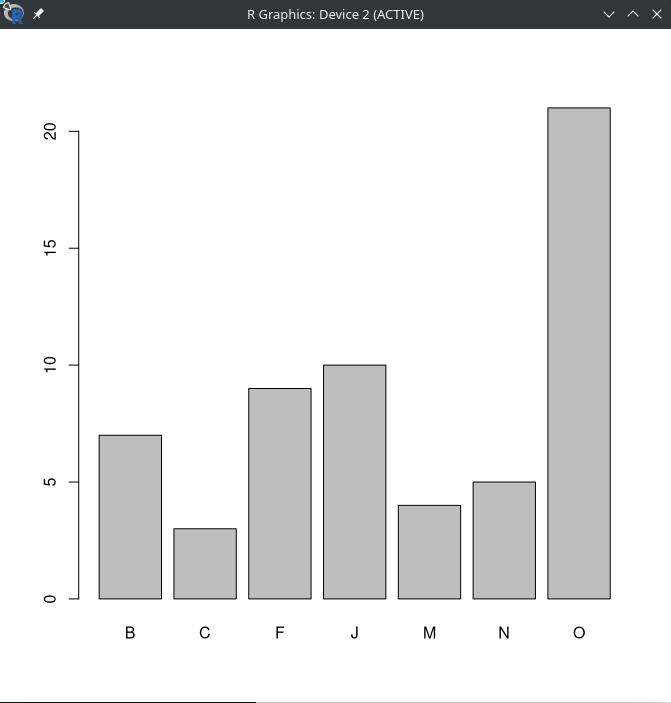
\includegraphics[width=.9\linewidth]{./imgs/h1p1.jpg}
\caption{\label{fig:org3170673}
Image contianing a barplot of the above frequencies}
\end{figure}

\subsection{Method/ Work Shown}
\label{sec:orgd49db7b}
I ran the following commands in R


\begin{verbatim}
data = c("O", "O", "N", "J", "C", "F", "B", "B", "F", "O", "J", "O", "O", "M", "O", "F", "F", "O", "O", "N", "O", "J", "F", "J", "B", "O", "C", "J", "O", "J", "J", "F", "N", "O", "B", "M", "O", "J", "M", "O", "B", "O", "F", "J", "O", "O", "B" , "N", "C", "O", "O", "O", "M", "B", "F", "J", "O", "F", "N")

sort(data)
data  // counted the data by hand to obtain the frequencies
data=c(B=7, C=3, F=9, J=10, M=4, N=5, O=21) //input the frequencies
data2 = data/59 * 100
data2 //this shows the relative frequencies
barplot(data)
\end{verbatim}

\section{Problem 2:}
\label{sec:orgcd709b0}
Blood pressure values are often reported to the nearest 5 mmHg (100, 105, 110, etc.). Suppose the actual blood pressure values for nine randomly selected individuals are 118.6 127.4 138.4 130.0 113.7 122.0 108.3 131.5 133.2

a. What is the median of the reported blood pressure values?
b. Suppose the blood pressure of the second individual is 127.6 rather than 127.4 (a small change in a single value). How does this affect the median of the reported values?

\subsection{Part a)}
\label{sec:orgeb06d06}
The median of the above set is 127.4

\subsection{Part b)}
\label{sec:org12a10d5}
The median is changed to be 127.6. This is because in both sets (be it 127.4 or 127.6) this number is the middle number when the set is sorted.

\subsection{Method}
\label{sec:org1b76952}
I ran the following commands in R. Some commands are added to support my claims.

\begin{verbatim}
data=c(118.6, 127.4, 138.4, 130.0, 113.7, 122.0, 108.3, 131.5, 133.2)
// init data for part a
sort(data)
median(data)
data //print the data to check work

data2=c(118.6, 127.6, 138.4, 130.0, 113.7, 122.0, 108.3, 131.5, 133.2)
// new data for part b
sort(data2)
median(data2)
data2
\end{verbatim}

\section{Problem 3}
\label{sec:orgfb90866}
Exposure to microbial products, especially endotoxin, may have an impact on vulnerability to allergic diseases. The article “Dust Sampling Methods for Endotoxin—An Essential, But Underestimated Issue” (Indoor Air, 2006: 20–27) considered various issues associated with determining endotoxin concentration. The following data on concentration (EU/mg) in settled dust for one sample of urban homes and another of farm homes was kindly supplied by the authors of the cited article.

U: 6.0 5.0 11.0 33.0 4.0 5.0 80.0 18.0 35.0 17.0 23.0
F: 4.0 14.0 11.0 9.0 9.0 8.0 4.0 20.0 5.0 8.9 41.0 9.2 3.0 2.0 0.3

\textbf{a. Determine the sample mean for each sample. How do they compare?}
\textbf{b. Determine the sample median for each sample. How do they compare? Why is the median for the urban sample so different from the mean for that sample?}
\textbf{c. Calculate the sample variance for each sample.}
\textbf{d. Make boxplots for each group and check to see if there is any outlier. If yes, what kind of outlier?}

\subsection{Part A)}
\label{sec:org07fd9bd}
The mean for the Urban set is : 21.54
The mean for the Farm  set is : 9.89

\subsection{Part B)}
\label{sec:org5f9c7b3}
The median for the Urban set is : 17
The median for the Farm  set is : 8.9

\subsection{Part C)}
\label{sec:org12d672f}
The variance for the Urban set is : 497.27
The variance for the Farm  set is : 99.27

\subsection{Part D)}
\label{sec:orgf4cf8b5}

\subsection{Work Shown}
\label{sec:org1b1dda8}
The below is a screen dump from my R konsole.

\begin{verbatim}
> Urban = c(6.0, 5.0, 11.0, 33.0, 4.0, 5.0, 80.0, 18.0, 35.0, 17.0, 23.0)
> Farm = c(4.0, 14.0, 11.0, 9.0, 9.0, 8.0, 4.0, 20.0, 5.0, 8.9, 41.0, 9.2, 3.0, 2.0, 0.3)
> mean(Urban)
[1] 21.54545
> mean(Farm)
[1] 9.893333
> median(Urban)
[1] 17
> median(Farm)
[1] 8.9
> var(Urban)
[1] 497.2727
> var(Farm)
[1] 99.26924
\end{verbatim}
\end{document}
